\section{Copyright}
\subsection{Patent, copyright and trademark}
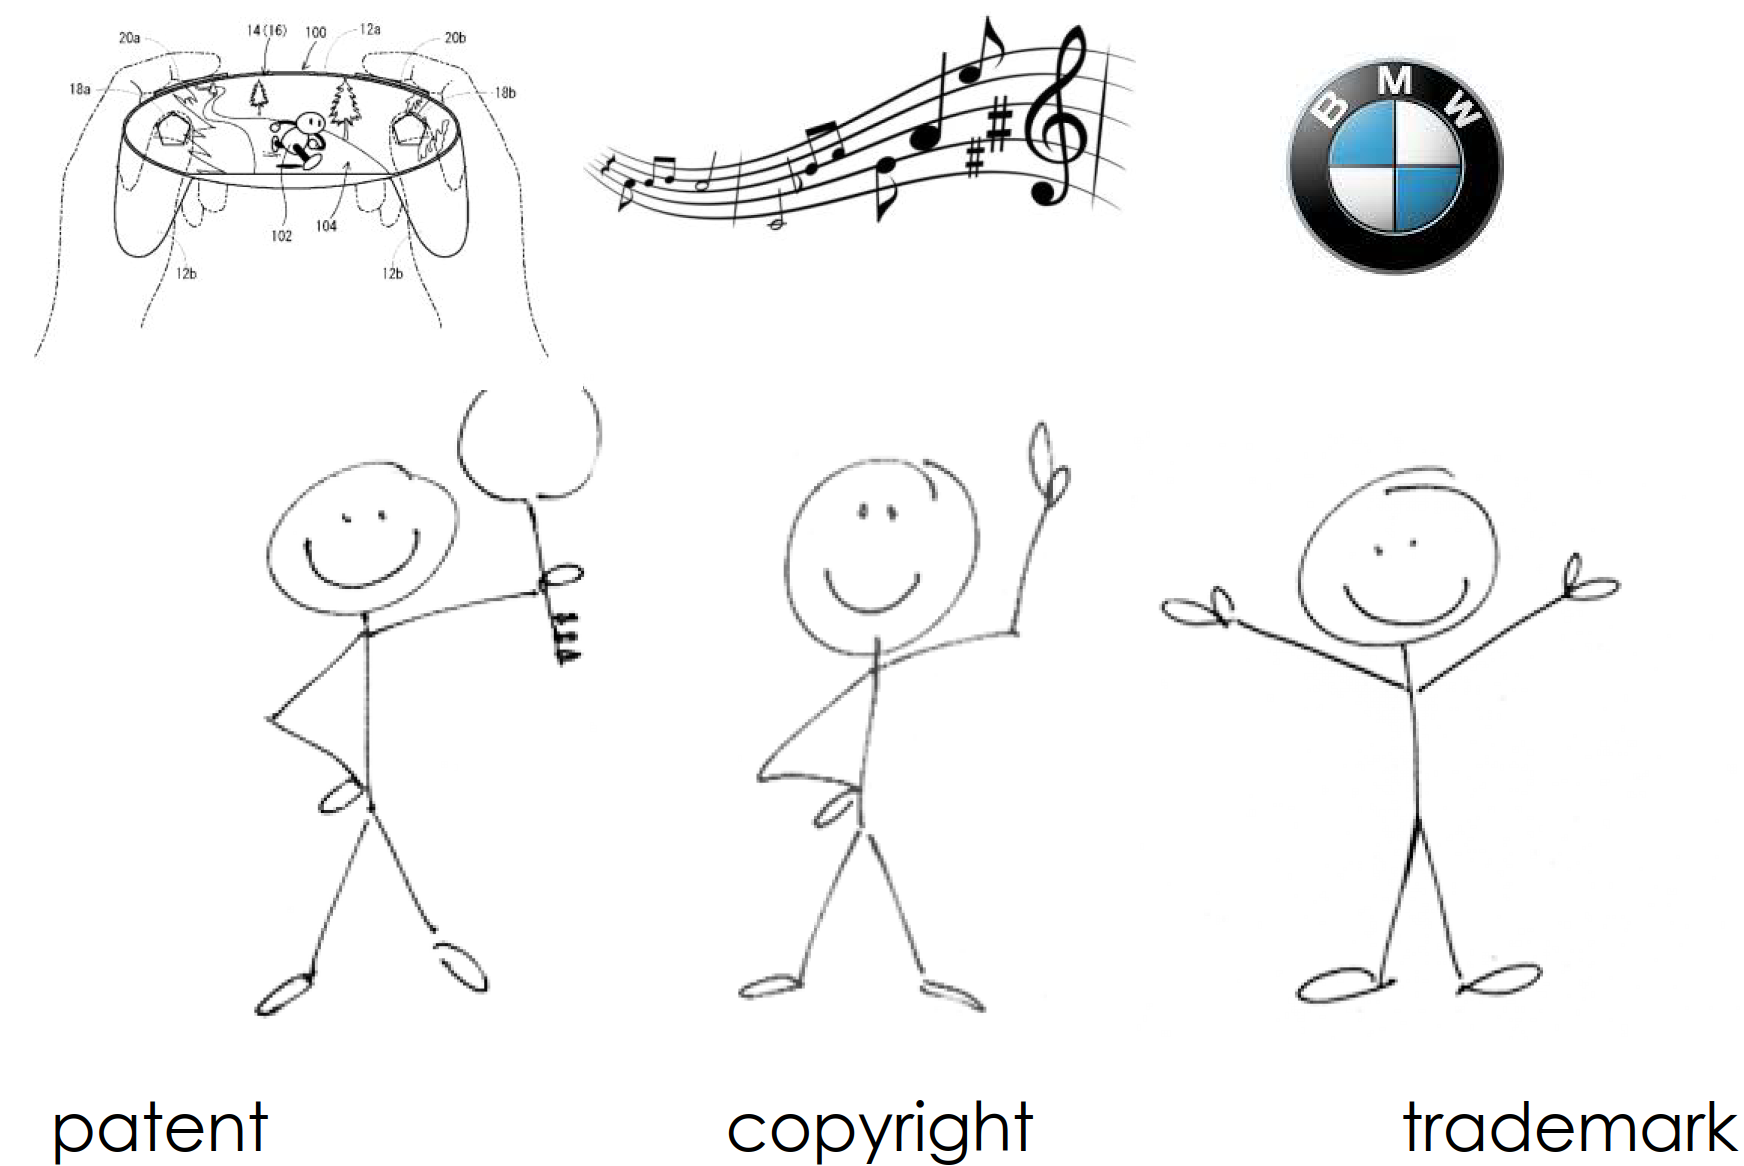
\includegraphics[width=1\linewidth]{images/patent_copyright_and_trademark}
Protection is limited to the form expressing an idea. Ideas as such or a mere concept are not protected. Ideas need to flow freely!

\subsection{Purpose of copyright law}
Through their works and performances, creative artists contribute to our country's cultural diversity . However they also want to earn something with their works and performances.
\begin{compactitem}
	\item The copyright law guarantees them financial remuneration for the utilization of their works. 
	\item The copyright law protects artists intellectual property in that they are able to defend themselves against misappropriation of their work.
	\item Copyright is a tool with which to earn something from cultural creativity. It is thus a part of our liberal economic and social order which safeguards property (including intellectual property). 
\end{compactitem}

\subsection{Definition of a "work"}
\begin{compactitem}
	\item Texts
	\item Music
	\item Photography
	\item Works of fine art
	\item Works with scientific content
	\item Architecture
	\item Visual and audiovisual works
	\item Choreographies and pantomimes
	\item Computer programs
\end{compactitem}

\subsection{Prerequisites for legal protection of a work}
\textbf{Prerequisites for legal protection:}
\begin{compactitem}
	\item Intellectual creation
	\item Individual character
	\item Perceptability / expression of an idea
	\item Irrespective of any value or purpose
	\item Work created by humans
\end{compactitem}
\textbf{“Statistical Uniqueness”, abstract criteria:}
\begin{compactitem}
	\item Characteristic features
	\item No one else would have created the work that way
	\item Sufficiently creative step beyond sheer otherness
	\item Work is something unique and special
\end{compactitem}
\textbf{Individual character:} \\
Analysis of concrete criteria for each category of work, eg photography
\begin{compactitem}
	\item Selection of object, image section and time of triggering
	\item Design of the image components
	\item Distribution of light and shadow
	\item Use of specific lenses or filters
	\item processing of the negative
\end{compactitem}

\subsection{Work and work copy}
Work: Intangible good / intellectual property (eg. Firefox)\\
Work copy: materialized work, ie physically existent, often (but not necessarily) physical expression of the work (eg. Firefox installed on a computer)

\subsection{Second hand work}
\begin{compactitem}
	\item Creation using pre-existing works
	\item Independent protection of these works, if protection requirements fulfilled
	\item Protection of the existing works is reserved
	\item Creative change of a pre-existing work
	\item Individual character and thus independent protection of processing. But: individual character of the existing work still recognizable
	\item Example: Translation, filming, staging
\end{compactitem}

\subsection{What is copyright?}
\begin{compactitem}
	\item Author of a copyrighted work is always the natural person who created the work (“creator principle”). Copyright law is an absolute right and thus excludes every other person.
	\item Copyrights can be transferred from the original author to another person/legal entity who then becomes the right holder.
\end{compactitem}

\subsection{Moral rights}
\begin{compactitem}
	\item Recognition of authorship
	\item First publication
	\item Integrity of the work
\end{compactitem}
Moral rights vest in the author and cannot be transferred/licensed.

\subsection{Authorship}
\textbf{Joint Authors:} \\
When multiple people work together pursuant to a common concept to create a work together. The joint authors can only decide jointly on what happens with the work. Conclude a contract! \\
\textbf{Copyright and Employment:} 
\begin{compactitem}
	\item General rule: the author is right holder upon creation. The employer is not entitled unless employee transfers the copyrights within individual employment contracts.
	\item Exception: the law assumes that copyright in a computer program vests in the employer if an employee creates the computer program during working hours as part of his or her job.
\end{compactitem}

\subsection{Duration of copyright}
A work is protected under copyright as soon as it is created . It is not necessary to file for protection or to “deposit” the work. In Switzerland there is no register.\\
\textbf{Not required:}
\begin{compactitem}
	\item Having the work recorded on a carrier (printed book, pressed CD)
	\item Publication of the work
	\item The explicit will to create work
	\item Ability to act: authors can, for example, also under-assisted or hypnotized persons
\end{compactitem}
\textbf{Formalities:} \\
It is also not necessary to refer to the copyright in the work. Notations such as “copyright“, “all rights reserved“ or “©” have no influence on protection in Switzerland. In other countries the notification can be important for copyright protection. \\
\textbf{Duration:}
In Switzerland copyright protection expires 70 years after the death of the author. Exception: the protection for computer programs ends 50 years after the death of the author.

\subsection{Limitations of copyright}
Whoever publishes, reproduces, performs, broadcasts or otherwise disseminates a work requires the author’s consent. However: Private use is not subject to license fees. But that does not apply to computer programs: Permission from the rights holder must be obtained for each use!

\subsection{Related rights}
The Copyright Act also regulates related rights (or neighboring rights).
\begin{compactitem}
	\item the rights of performing artists (musicians, actors) to their performances;
	\item the rights of producers of phonograms and videograms to their products (CD, DVD);
	\item the rights of broadcasters to their radio and television broadcasts.
\end{compactitem}
Related rights protection expires 50 years after the performer’s performance, the publication of the phonogram or videogram (or the production of it, in the case that it is not published) or the emission of the broadcast. The rights of a performing artist to be named as performer ends upon his or her death, or 50 years after the performance, at the earliest.

\subsection{Legal protection}
\textbf{Civil procedures:} \\
Civil proceedings involve copyright claims between private persons/private legal entities.
The author/right holder can request from the civil court
\begin{compactitem}
	\item a declaratory judgment (have a right established);
	\item have an infringement banned/remedied;
	\item have property confiscated;
	\item have an order published.
\end{compactitem}
\textbf{Criminal procedures:} \\
Criminal procedures may be initiated by the right holder within 3 months after becoming aware of an infringement or the authorities. \\
Fines or imprisonment of up to 1 year (or 5 years if committed on a commercial basis) for use without the right holder’s consent in particular:
\begin{compactitem}
	\item use of a work within correctly indicating the author
	\item publishing a work
	\item change a work
	\item use for derivative work
	\item copies of works
	\item distributing or making works available
	\item broadcasting
	\item renting out of computer programs
\end{compactitem}

\subsection{Collecting Societies}
The Federal Copyright Act is based on the view that the rights accruing to authors are essentially the responsibility of the right holders to assert for themselves. The Federal Copyright Act only envisages collective management by collective rights management organizations in circumstances where mass utilization makes direct management virtually impossible.

\subsection{Copyright law and Internet}
\textbf{Use of content:} \\
Downloading, copying, scanning, etc., are types of use of a copyrighted work. \\
The right holder has the right to give permission to any kind of use of his work or to revoke this permission. This permission must be given expressly (verbally or in writing) or implied. \\
When published works are used as sources in the Internet, they must be cited in the way books are cited; otherwise plagiarism is taking place. \\
\textbf{Links:} \\
This first of all facilitates access to the linked page (by clicking directly on the link), and secondly implies to the internet user that the linked pages are associated. This assumption can be wrong. Therefore, rights can in fact be infringed simply through linking, such as those contained in the Federal Act against Unfair Competition (UCA) or the Data
Protection Act (DPA). Therefore, linking should always be agreed upon between the parties.

\subsection{Federal copyright act}
The Federal Copyright Act of 1992, is the legal basis for the protection of literary works and works of art. It is currently under revision. It also governs what are known as “neighboring rights”, i.e. the rights of performers, record producers and broadcasting companies. The Federal Copyright Act stipulates the rights and obligations of the five
collective administration societies.